\section{Introduktion}
\begin{itemize}
	\item Implementeret i network interface card'et (NIC)
	\item Framing
	\item Checksum
	\item Errorhandling (Ethernet vs. WiFi)
	\item Nodes \& links
\end{itemize}

\section{Multiple Access}
\begin{itemize}
	\item Point-to-point link
	\item Broadcast link
	\item Multiple access problemer
\end{itemize}

\subsection{Protokoller}
\begin{itemize}
	\item Channel partitioning protocols (CDMA)
	\item Random access protocols (aloha, slotted aloha, CSMA)
	\item Taking-turns protocols (polling protocol, token-passing protocol)
\end{itemize}

\section{Error detection \& correction}
\begin{itemize}
	\item Checksum: Error detection bits
	\item Modtager kontrollerer frame for fejl
	\item Afhængig af link-lags protokol kasseres eller rettes frames med fejl
\end{itemize}

\section{Link layer addressering}
\subsection{MAC}
\begin{itemize}
	\item Media Access Control
	\item 48 bit MAX adresse (NIC kort)
	\item Administreret af IEEE (the Institue of Electrical and Electronics Engineers)
	\item Flytbar
\end{itemize}

{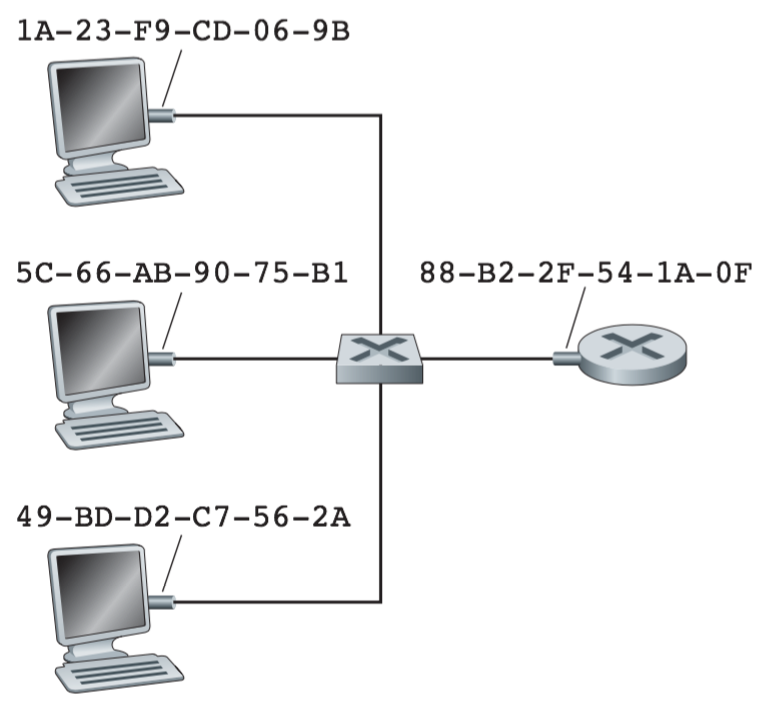
\includegraphics{5-data-link-layer/mac.png}

\subsection{ARP}
\begin{itemize}
	\item Address Resolution Protocol
	\item Mapper ip-addresser til MAC adresser
\end{itemize}

{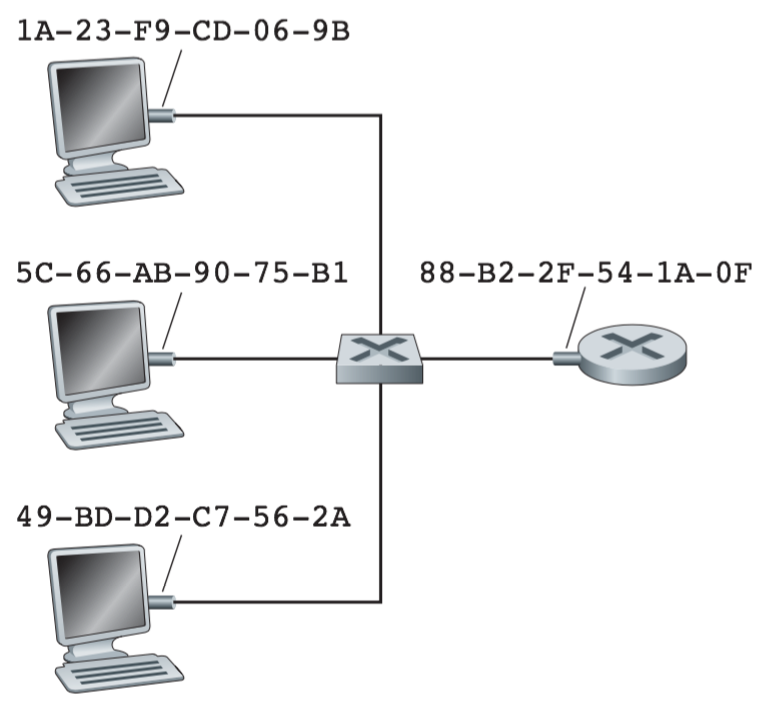
\includegraphics{5-data-link-layer/mac.png}

\section{Ethernet}
\begin{itemize}
	\item Mest udbredte LAN teknologi
	\item Frame struktur
\end{itemize}

{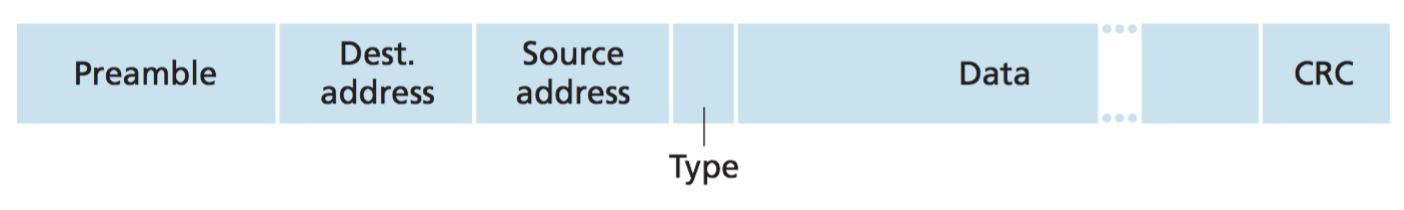
\includegraphics[scale=0.6]{5-data-link-layer/ethernet.png}